\section{Auswertung}
\subsection{Bestimmung der Relaxationszeit}  %--> idk wie wir layout mache wollen/section gerüst usw
Zur Bestimmung der vorher definierten Relaxationszeit $\tau = RC$ wird der Entladungsvorgung des Kondensators untersucht.
Dazu werden die gemessenen Spannungen $U_{C}$ bei entsprechender Zeit $t$ in einem halblogarithmischen Diagramm dargestellt.
Anschließend folgt die Annährung einer linearen Ausgleichsgerade durch Python, mit einem charakteristischen Steigungsparamter $a$
der Form $1/RC$. 
Die ermittelte Ausgleichsgerade hat also die Form.
\begin{equation}
    \text{ln}(U_{C}(t)) = a \cdot t + b
\end{equation}
Die Parameter der Gerade lauten.
 \begin{align*}
     a &= \SI{-804.325(52531)}{\si{\per\second}} \\
     b &= \SI{0.950(123)}{}
 \end{align*}
Der Vergleich mit der Gleichung \eqref{eqn:gerade} zeigt nochmal die Verbindung zwischen $a$ und $\tau$. Die Relaxationszeit ist folglich.
\begin{equation}
\tau = RC = - \frac{1}{a} = \SI{1.24(8)}{\milli\second}
\end{equation}
 
\begin{figure}
    \centering 
    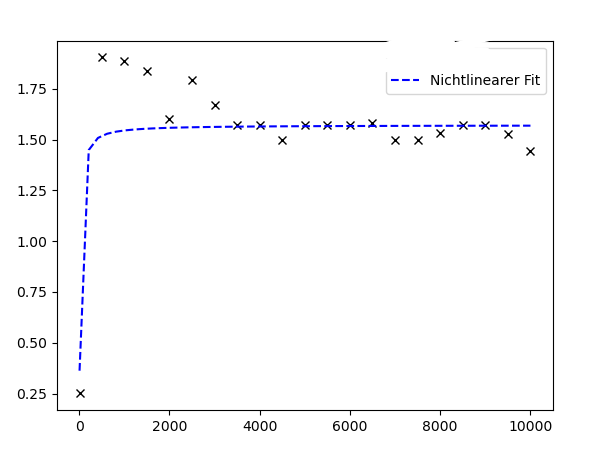
\includegraphics[width=\textwidth]{build/plot1.pdf}
    \caption{Messwerte der Entladungskurve in halblogarithmischer Darstellung mit Ausgleichsgeraden.}
    \label{plt:plot1}
\end{figure} 
